\chapter{Architecture}
% OR: \chapter{Model}
\label{cha:architecture}

\begin{comment}
Here you will present the architecture or model that you have chosen and which is (or will be) implemented in your work.
Note that putting algorithms in your report is not always desirable, so in certain cases those might be placed in the appendix.
Code is normally to be avoided in the report itself, but may be included in an appendix or submitted as additional documents.
(The actual code must also be submitted together with the final Master's thesis, but as a zip-file.)

Any off-the-shelf tools and methods that you use in your architecture should have been introduced earlier,
tentatively in the Background chapter (or in the Related Work chapter),
so that they can be referenced here by giving backward pointers to the previous text.

Here, or in a separate chapter (or possibly in the Background chapter or in the Experimental Setup),
you should also discuss the data that you use in your experiments (see Chapter~\ref{cha:data}).

\textit{Nunc in tristique risus, ut malesuada tortor. Integer ullamcorper nunc a felis vehicula condimentum. Aliquam eget turpis purus. Nam nec ipsum sed ligula vulputate tempor ac non arcu. Aenean hendrerit pretium ante et suscipit. Proin vitae venenatis ex, at pellentesque erat. Nulla facilisi. Sed quis eros lorem. Praesent id pharetra risus. Nunc a lacinia est. Nunc in urna at purus ullamcorper blandit eget sit amet est. Cras sagittis et ante ut lobortis. Proin quis arcu eros. Aliquam tempor neque vehicula lacus placerat, ac ultricies massa ultricies. Aliquam et nulla eget felis accumsan rutrum quis sed ligula.}

\textit{Vivamus bibendum tempus tincidunt. Integer imperdiet lectus pellentesque, rhoncus quam at, tempor ex. Phasellus semper tempor sapien at consequat. Proin ut dolor interdum, ullamcorper leo ac, convallis metus. Nullam tincidunt, metus ullamcorper sodales placerat, ipsum ipsum porttitor est, id volutpat orci orci sit amet quam. Vestibulum sagittis urna sit amet nulla vulputate, nec pellentesque enim hendrerit. Suspendisse at laoreet ipsum. Phasellus arcu nisi, laoreet sed tellus sit amet, imperdiet fringilla ante. Quisque rhoncus accumsan magna vel posuere. Fusce facilisis est eros, ac viverra diam maximus ut. Nullam ut lectus nunc. Fusce vestibulum sem at ex euismod tempus. Lorem ipsum dolor sit amet, consectetur adipiscing.}

\textit{Phasellus sed ipsum nunc. Nam iaculis felis mauris, sit amet condimentum ex malesuada at. Morbi lacinia odio mi, sit amet pellentesque ante facilisis sit amet. In lobortis elit ut dictum mollis. Aliquam erat volutpat. Morbi sit amet metus nisi. Nulla auctor varius metus at rhoncus. Pellentesque porta mollis leo, eu ultricies nulla mollis ac. Vivamus interdum ac odio vitae sodales. Aenean finibus eros rhoncus molestie elementum. Integer maximus erat vitae purus lobortis iaculis. Etiam blandit varius nulla, sed euismod felis.}

Clearly, a figure showing the architecture is a must, such as Figure~\ref{fig:Architecture}.
Describe all parts of such a figure in reasonable detail in the text, possibly with forward pointers to sections where they will be elaborated on (or backward pointers to sections where tools and methods already have been introduced).
Mention work that motivated your architectural choices, parameter settings, etc.
Those choices should then also be discussed and elaborated on in the Discussion chapter.

\begin{figure}[t!]
    \centering
    \missingfigure{Architecture figure to be added}
    \caption{The missing architecture}
    \label{fig:Architecture}
\end{figure}
\end{comment}

The \nameref{cha:architecture} chapter will give a detailed description of the inner workings of GeoGPT, the thesis' proposed solution to an \acrshort{acr:llm}-based \acrshort{acr:gis}. GeoGPT is a webpage that features a chat interface and a web map, where users can ask questions and receive answers as text and/or map geometries. \Autosectionref{sec:high-level-application-architecture} will present a high-level overview of the different modules that make up GeoGPT, and the way that they interact with each other. \Autosectionref{sec:agent-architecture} will delve into the architecture of the generic tool agent that is implemented using LangChain and LangGraph (see \autoref{sec:langchain} for detailed information), as well as the \textit{three} different agent types that are implemented using this generic agent.

\section{High-Level Application Architecture}
\label{sec:high-level-application-architecture}

A microservice architecture was adopted to simplify development and separate concerns among the system's different functionalities. The services are deployed as Docker Containers, and are orchestrated using Docker Compose. \autoref{fig:architecture-overview} shows how the application is divided into five distinct services, and shows the general direction of information flow between these. \autoref{fig:sequence-diagram} goes into greater detail, showing how the different services interact with each other when the user first loads GeoGPT and enters a question into its chat interface.

\begin{figure}[h]
    \centering
    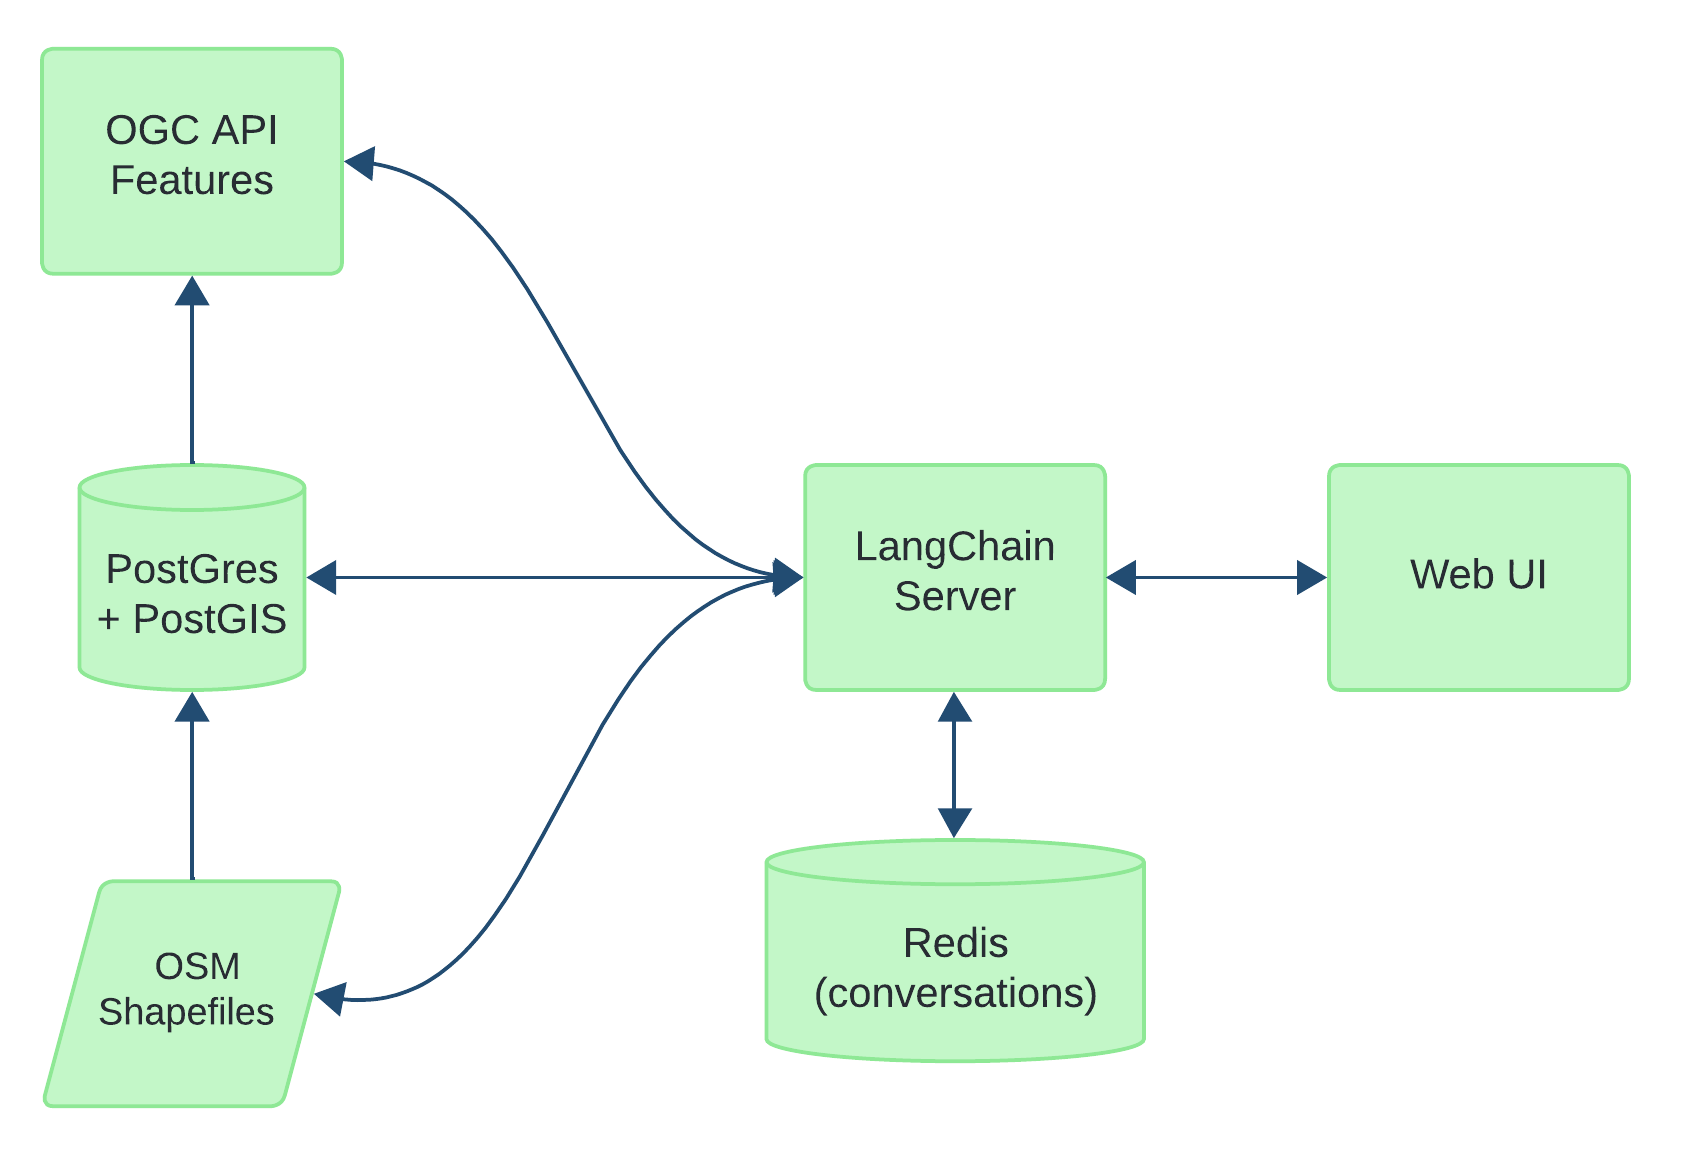
\includegraphics[width=\textwidth]{microservices.png}
    \caption{Architecture overview}
    \label{fig:architecture-overview}
\end{figure}

\begin{figure}
    % \centering
    \makebox[\textwidth][c]{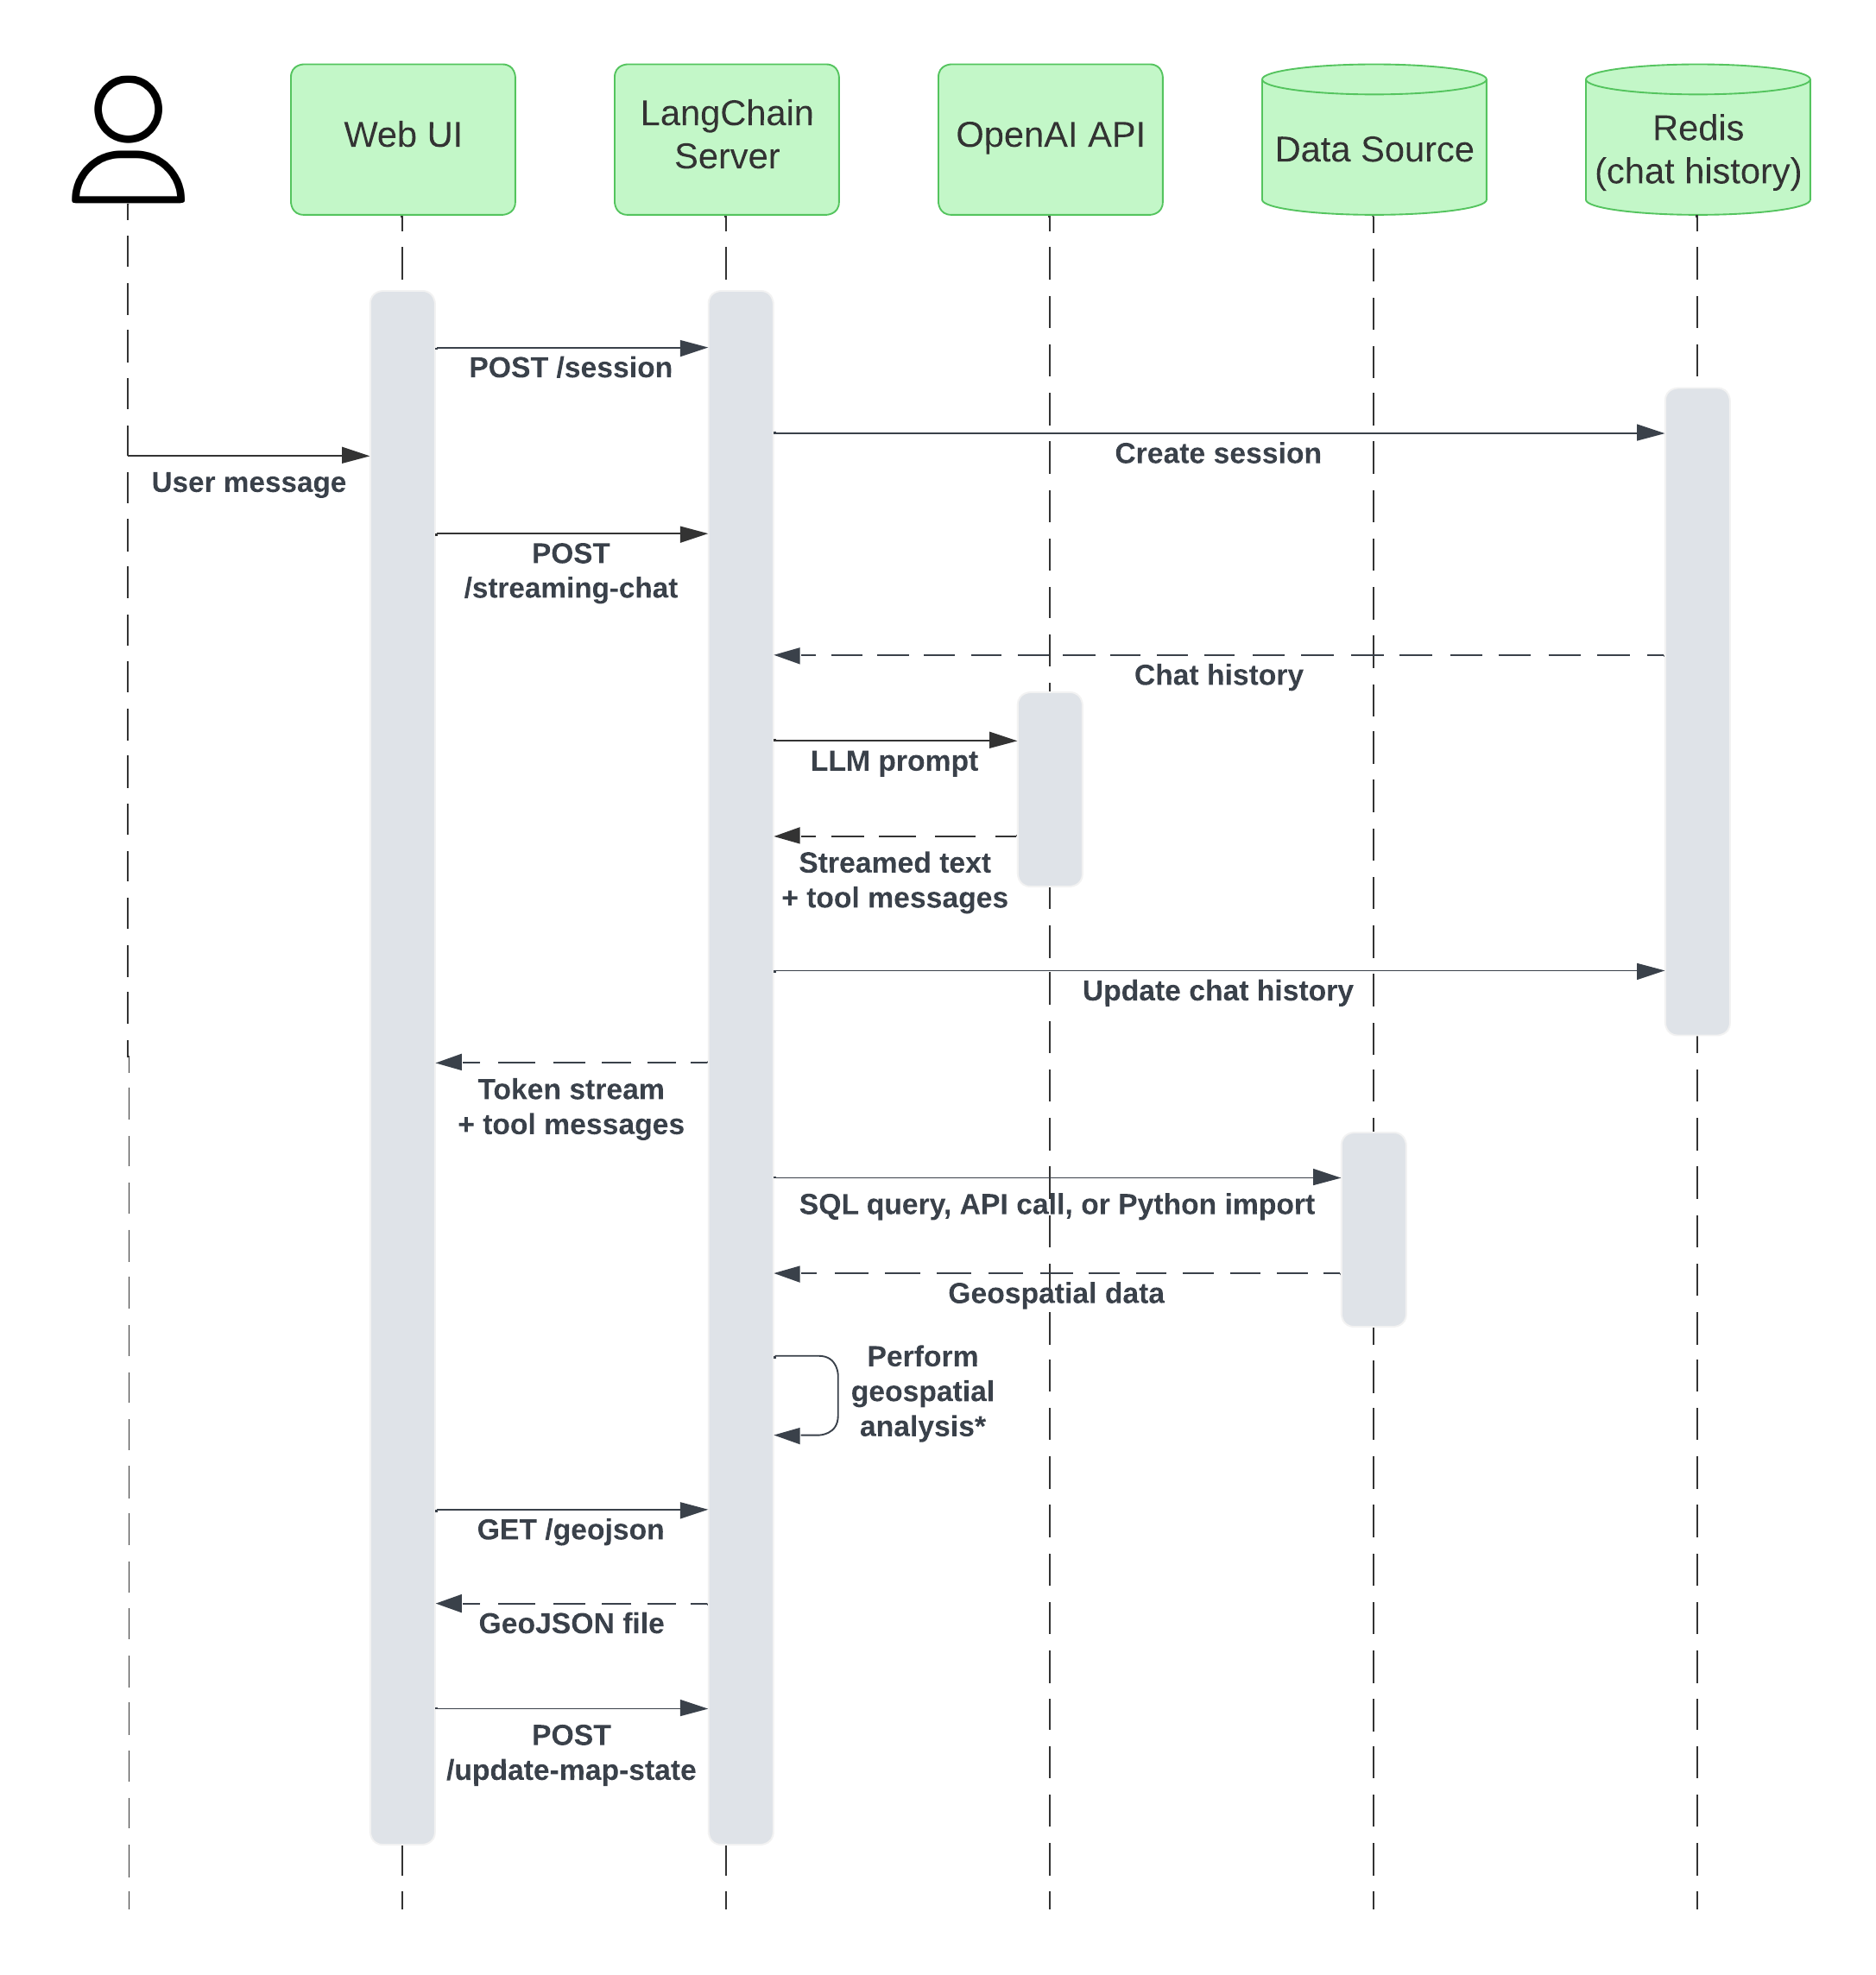
\includegraphics[width=1.2\textwidth]{Sequence diagram.png}}
    \caption{Sequence diagram showing the information flow as the user loads and sends a message to GeoGPT}
    \label{fig:sequence-diagram}
\end{figure}


\subsection{LangChain Server}\label{subsec:langchain-server}

The \textit{LangChain Server} service is the heart of the application, and is where the \gls{acr:llm}-related logic is situated. It is responsible for taking requests from the \textit{Web \acrshort{acr:ui}} and returning suitable responses in what becomes a client-server architecture between the two services. \autoref{tbl:server-endpoints} shows the endpoints exposed by the server and how they can be used by a client.

\begin{table}[H]
    \centering
    \caption{Summary of Server Endpoints}
    \label{tbl:server-endpoints}
    \begin{tabular}{p{0.22\textwidth}p{0.1\textwidth}p{0.55\textwidth}}
        \toprule
        \textbf{Endpoint} & \textbf{Method} & \textbf{Description}                                                                                                                                                         \\
        \midrule
        /session          & GET             & Takes a \texttt{session\_id} as a query parameter, allowing the client to continue on a pre-existing session.                                                                \\
        /session          & POST            & Creates a new session with an empty conversation.                                                                                                                            \\
        /streaming-chat   & GET             & Endpoint for chatting the \acrshort{acr:llm}. Takes a \texttt{message} as a query parameter and returns an event stream, allowing for token streaming from server to client. \\
        /update-map-state & POST            & Send the state of the client map to the server. Keeps the server updated on what layers are present in the map, their color, etc.                                            \\
        /geojson          & GET             & Takes a \texttt{geojson\_path} as a query parameter. Allows the client to retrieve a given GeoJSON file that is stored in the working directory on the server.               \\
        % /history          & GET             & Used to retrieve the chat history of the current session.                                                                                                                    \\
        /upload           & POST            & Allows the client to upload one or more files to the working directory on the server.                                                                                        \\
        \bottomrule
    \end{tabular}
\end{table}


\subsection{Redis for Conversations}

Redis \citep{sanfilippoRedisRealtimeData2009} is a fast in-memory database that is often applied as a caching database that sits on top of some persistent database. It can also be used for vector-based storage, or as a simple NoSQL database. The latter option is the way it is used in GeoGPT's architecture, and its sole purpose is to store conversations between GeoGPT and its users. Whenever a user starts a conversation with GeoGPT, a session object is stored in the Redis database, as can be seen in \autoref{fig:sequence-diagram}. This object holds an array that represents the conversation. This array is written to every time the human, or GeoGPT, produces a message.

Storing messages, either in memory as a simple array or in a database like Redis, is crucial to enable multi-message conversations. In order for an \gls{acr:llm} to act as a conversational agent, a chat history needs to be included in the prompt. In the case of GeoGPT, the entire chat history is included. This has the advantage of providing the \gls{acr:llm} with the complete context of the chat history, but the disadvantage of potentially bloating the context window. Therefore, as the chat becomes longer each new token will be both more expensive and take longer to get generated. A long chat history could also make the resulting prompt exceed the token limit of the \gls{acr:llm}. These issues were not considered much for this project and are left for future work.

\subsection[PostGIS and OGC API Features]{PostGIS \acrshort{acr:ogc} \acrshort{acr:api} Features}

A PostgreSQL database with the PostGIS extension, containing the datasets in \autoref{app:datasets}, was deployed using Docker. On top of this database is an \acrshort{acr:ogc} \acrshort{acr:api} Features web server. It is realized through the \texttt{pramsey/pg\_featureserv} Docker image\footnote{\url{https://hub.docker.com/r/pramsey/pg_featureserv}} \citep{crunchydataCrunchyDataPg_featureserv2024}, which is simply passed a connection string to the PostGIS database one wishes to expose on as an \acrshort{acr:ogc} \acrshort{acr:api} Features server. Any tables in that database which have a geometry column and a specified \gls{acr:crs} will be exposed on the server. \textit{pg\_featuresserv} includes functionality like bounding box filtering, result limiting, and \acrshort{acr:cql} filtering. These are added as query parameters in the URL used to fetch a collection's items, for instance:

$$
    \texttt{.../collections/\{collection\_id\}/items.json?limit=1000\&filter=name IS NOT NULL}
$$

In the internals of \textit{pg\_featuresserv}, this URL will be converted to an \acrshort{acr:sql} query that will be run against the database. Results of the query will be returned as GeoJSON. \autoref{code:cql-to-sql} shows an example of how \acrshort{acr:cql} code is converted into \acrshort{acr:sql} code:

\begin{lstlisting}[
    language=SQL,
    label=code:cql-to-sql,
    caption=Conversion from \acrshort{acr:cql} to \acrshort{acr:sql}
]
\\ CQL code passed through the `filter` query parameter
within(geom, POINT(0 0))

\\ SQL code that will be run agains the database
ST_Within("geom",'SRID=4326;POINT(0 0)'::geometry)
\end{lstlisting}

\subsection[Web UI]{Web \acrshort{acr:ui}}

The user interface is made using SolidJS, a JavaScript framework for creating websites. The user interface is intentionally quite minimal, aiming to simplify the way we do \acrshort{acr:gis} analysis.

\begin{figure}[h]
    \centering
    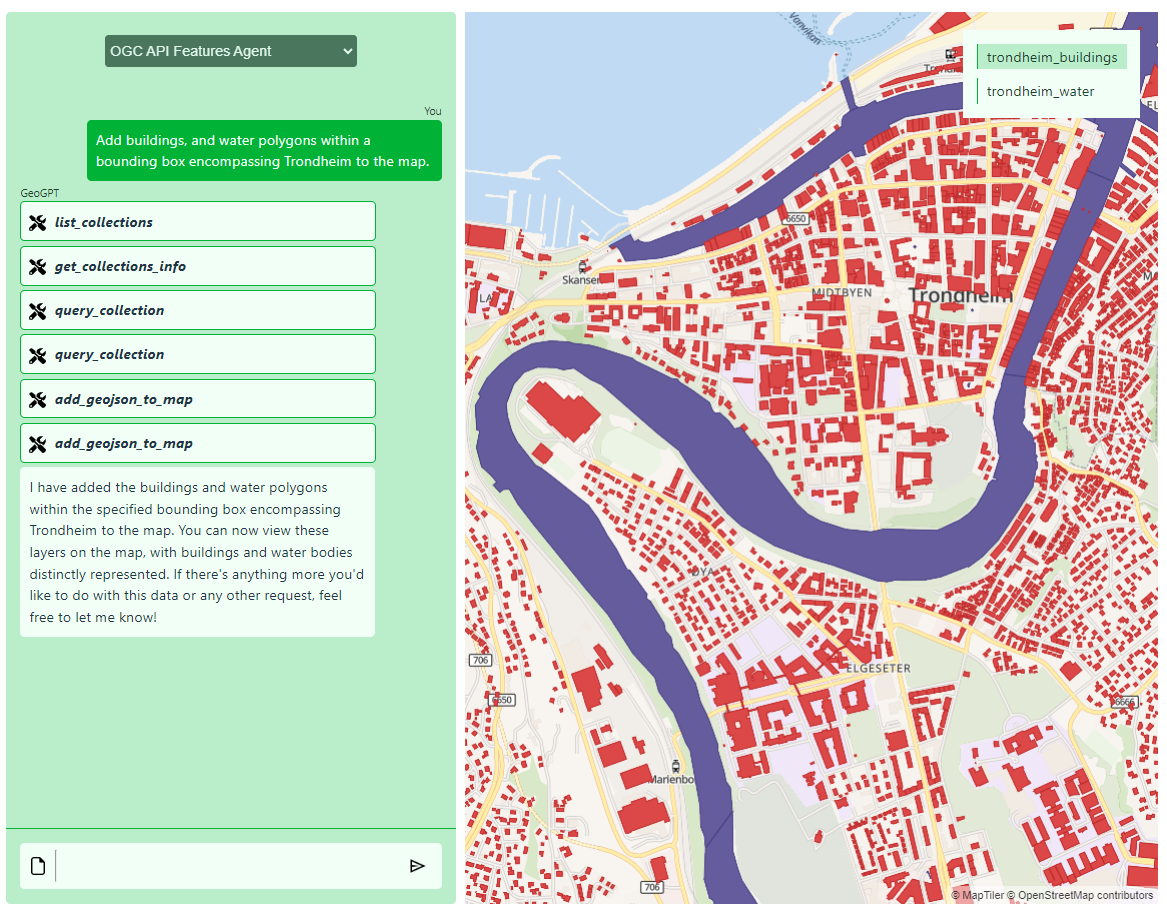
\includegraphics[width=\textwidth]{web_ui_overview_2.png}
    \caption{Web \acrshort{acr:ui}}
    \label{fig:web-ui}
\end{figure}

The chat interface was designed to imitate the interface of OpenAI's ChatGPT. Tokens and tool messages are streamed from the LangChain server, which helps the user follow GeoGPT's thought process as it is solving a problem. The generated text is streamed to the client token by token, and is in Markdown format. A library called \textit{showdown}\footnote{\url{https://github.com/showdownjs/showdown}} is used to convert Markdown into \acrshort{acr:html}, ensuring that tables, code blocks, lists, and other elements are properly rendered. Left of the input field on the bottom of the chat is a file upload button. Files that are uploaded here will be added to the working directory on the LangChain server.

The map is created using MapLibre,\footnote{\url{https://github.com/maplibre/maplibre-gl-js}} an open-source fork of Mapbox. A base map from \gls{acr:osm} is used, fetched through a mapping platform called MapTiler.\footnote{\url{https://www.maptiler.com/}} GeoJSON files that are fetched from the server will be added to the map automatically with a random color. On the top-right of the map is an overlay listing all layers that are currently present in the map. Using the arrow keys on this list will change the z-index in the map of the selected layer.


\section{Agent Architecture}
\label{sec:agent-architecture}

Three different agent were implemented for GeoGPT. These are listed below:

\begin{itemize}
    \item \textbf{\acrshort{acr:ogc} \acrshort{acr:api} Features Agent} -- Utilizes \acrshort{acr:ogc} \acrshort{acr:api} Features to interact with geographic data through standardized web interfaces.
    \item \textbf{Python Agent} -- Accesses and manipulates shapefiles using Python code, enabling detailed geographic data processing.
    \item \textbf{SQL Agent} -- Interacts with data stored in an \acrshort{acr:sql} database, allowing for complex queries and data management within GeoGPT.
\end{itemize}

Common to these agents is their agentic architecture, which is described in \autoref{subsec:lg-agent-implementation}. They differ, however, through their assigned \textit{tools}, which are described in \autoref{subsec:tools}. Other slight differences are seen in the way that they are prompted. The prompting strategy used for GeoGPT will be discussed in \autoref{subsec:prompt-templating}.

\subsection{LangGraph Agent Implementation}
\label{subsec:lg-agent-implementation}

The agentic behaviour of GeoGPT is implemented using LangGraph, which was described in detail in \autoref{sec:langchain}. \autoref{fig:tool-agent-graph} illustrates the flow between the various nodes that make up the agent. A state dictionary is passed between and updated by these nodes. Included in this state is the chat history, the path to GeoGPT's working directory, a list of the current files in this directory, as well as less important state. The implementation is based upon a prebuilt implementation from LangGraph.\footnote{\url{https://github.com/langchain-ai/langgraph/blob/main/langgraph/prebuilt/chat_agent_executor.py}}

\begin{figure}
    \centering
    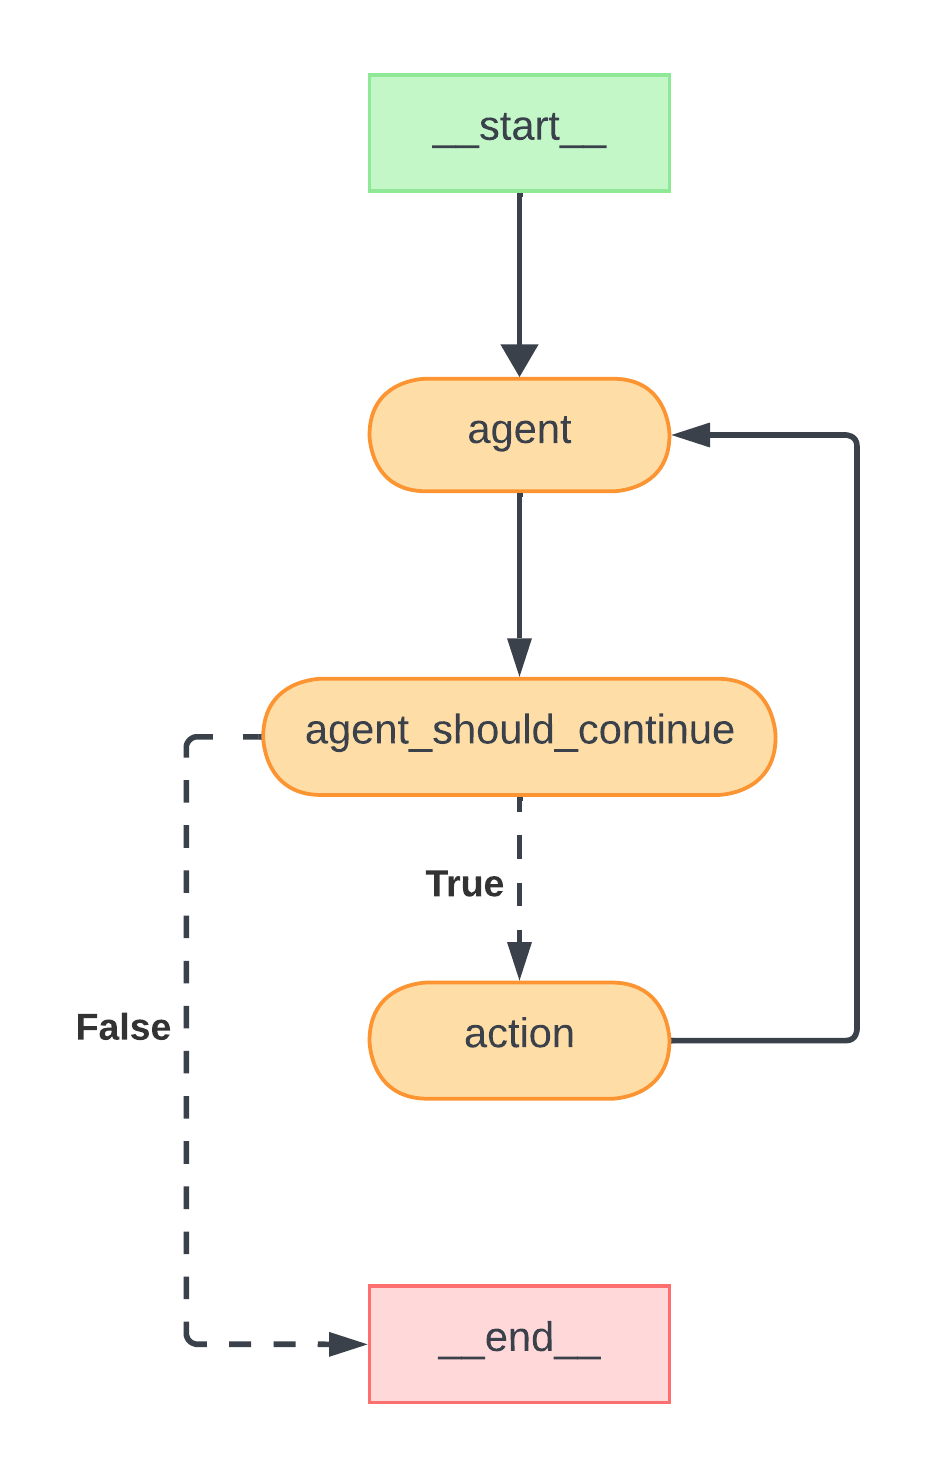
\includegraphics[width=0.6\textwidth]{agent_graph.png}
    \caption{Generic tool agent graph}
    \label{fig:tool-agent-graph}
\end{figure}

The \texttt{\_\_start\_\_} node serves as the entry point of the agent. At this point, only one message is present in the state, namely the initial message from the user. The \texttt{\_\_start\_\_} node points to the \texttt{agent} node, where a a prompt is constructed and passed to the \acrshort{acr:llama}, so that a response to the user can be generated. This response could contain a textual response, and/or instructions to execute some tool. For this reason, the current state containing both the user message and the \acrshort{acr:ai} message, is sent to the conditional node called \texttt{agent\_should\_continue}. This node simply checks if the last \acrshort{acr:ai} includes the \enquote{tool\_calls} keyword argument. If this is the case then some tool should be executed, and we should \enquote{continue}.

In the \texttt{action} node, the values attached to the \enquote{tool\_calls} keyword argument, which are \acrshort{acr:llm}-generated, are used to invoke predefined tools. The \acrshort{acr:llm} specifies tool \textit{names}, as well as tool \textit{parameters} that will be passed to the predefined tool (see \autoref{subsec:function-calling} for more details on how \textit{function/tool calling} works). These tools are then executed, possibly having side effects on the server, and the return values from the tools are appended as messages to the chat history. \autoref{fig:chat-trace-example} illustrates this behaviour. This way, the agent can inspect the outcome of these tool invocations, and be notified if there are any errors occur in the tools due to the parameters it passed. Through the cyclic behaviour of the agent graph the agent can repeatedly call tools to try and answer the request from the user. When the agent finds no reason to call any more tools, \texttt{agent\_should\_continue} will return \texttt{False} so that the termination node, \texttt{\_\_end\_\_} is reached.

\begin{figure}
    \centering
    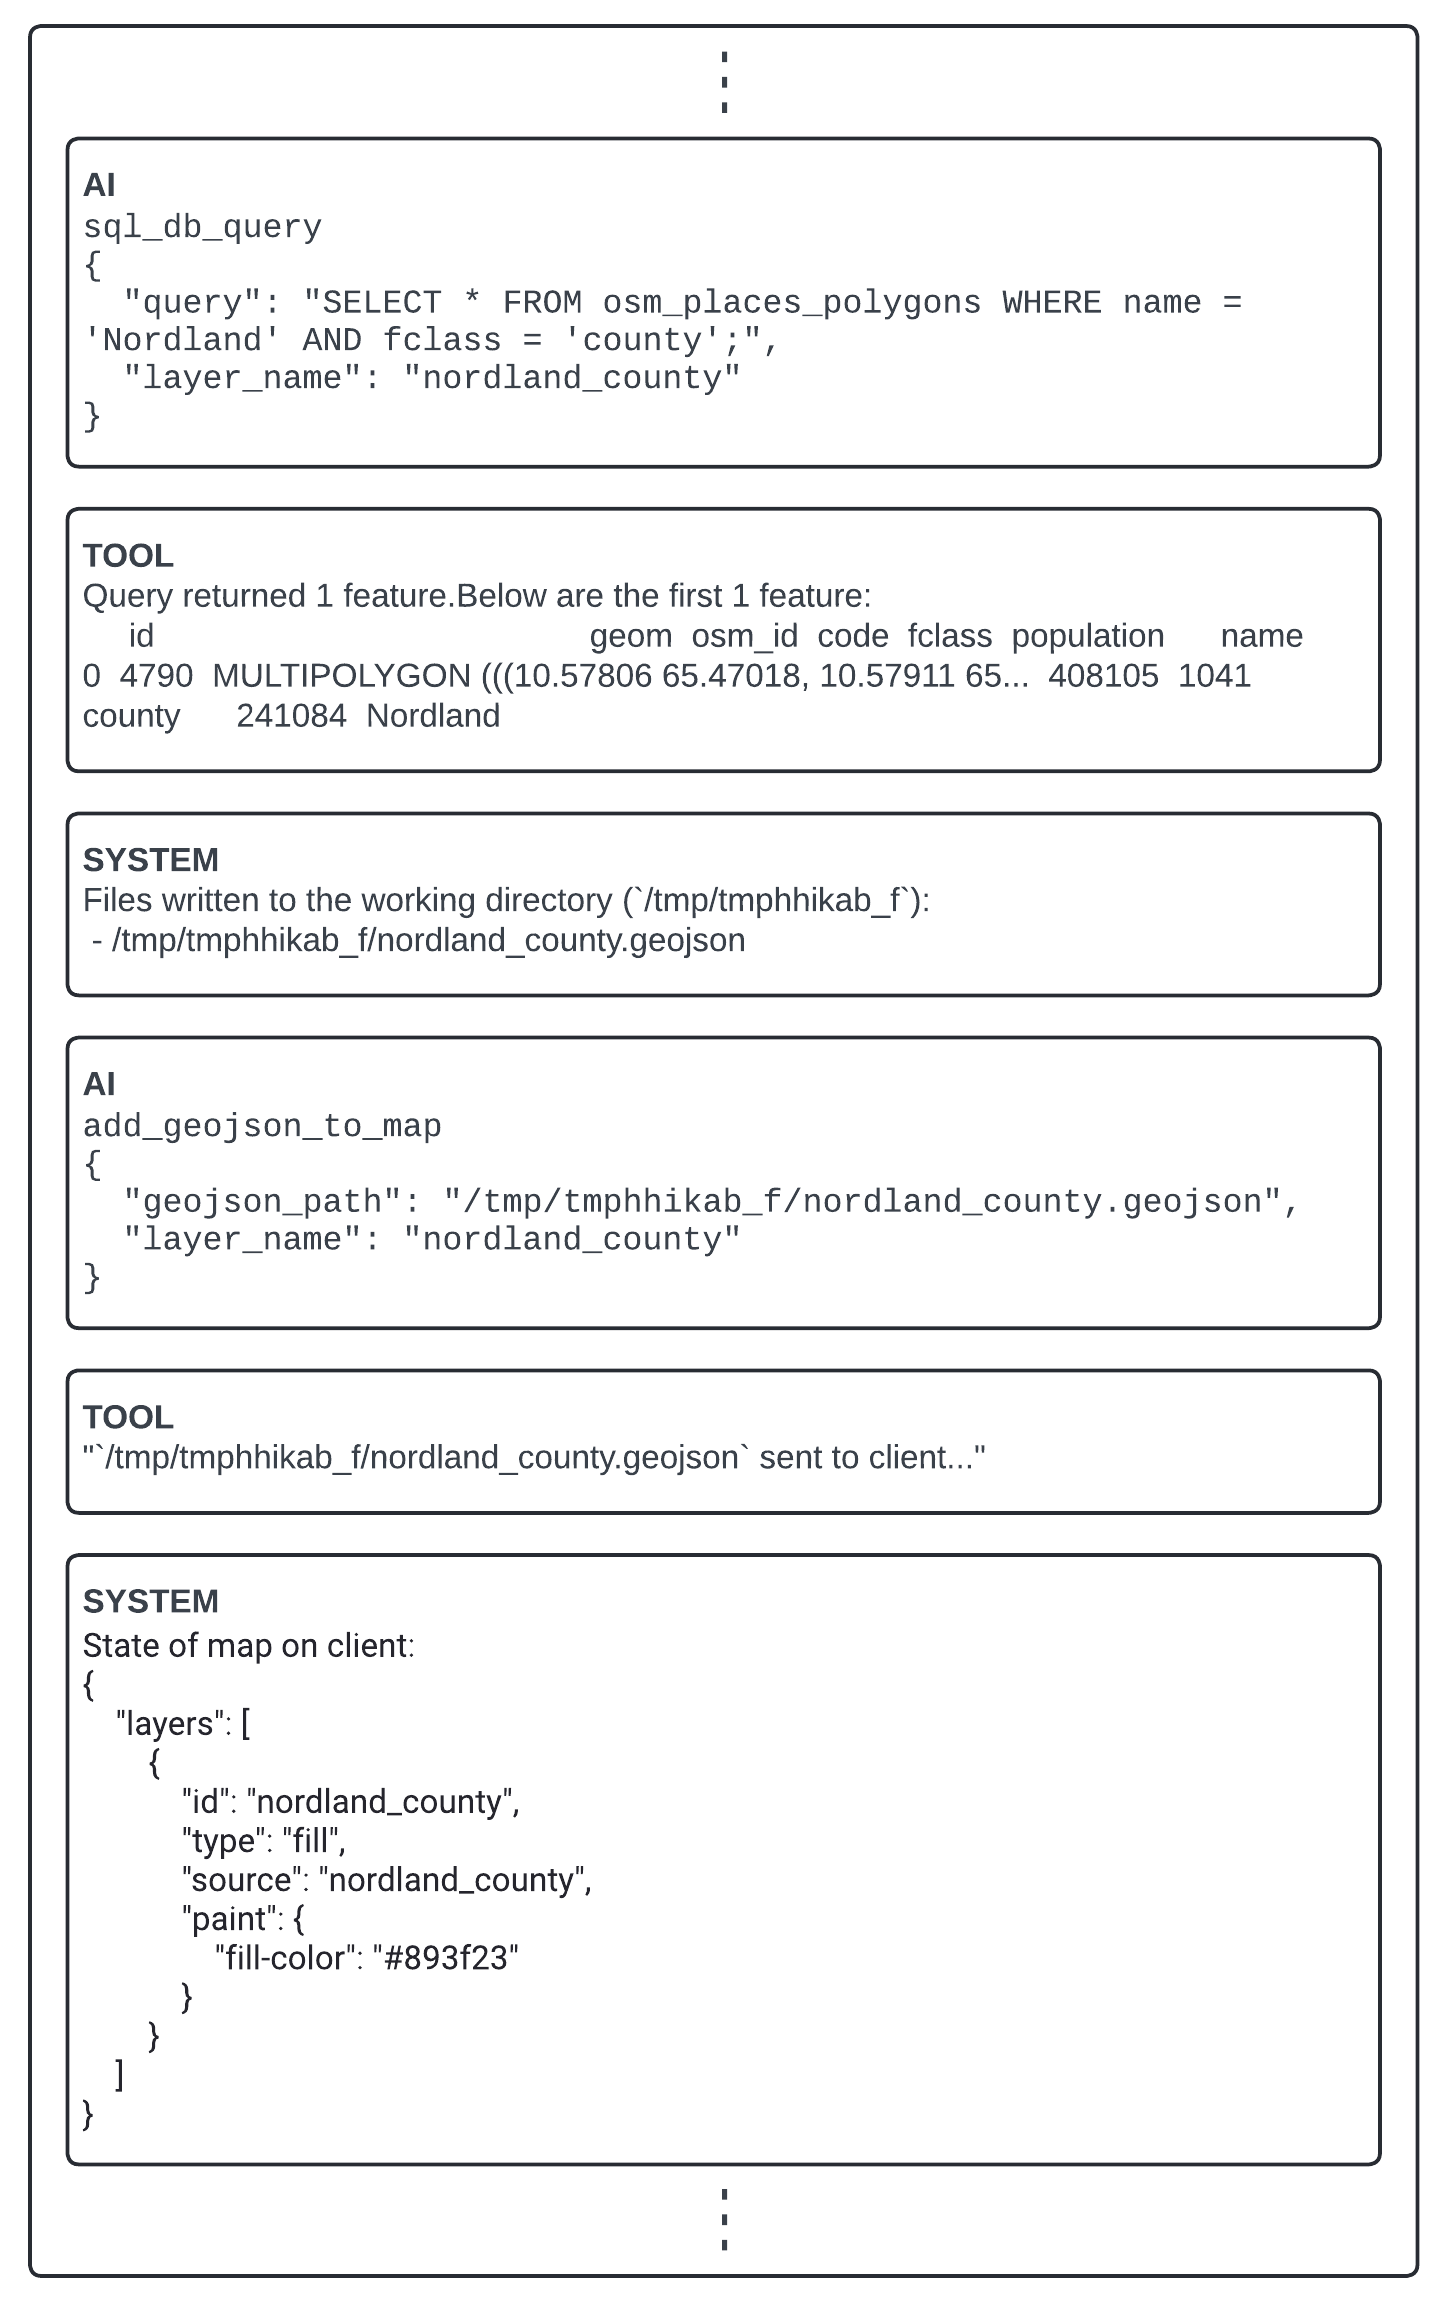
\includegraphics[width=0.9\textwidth]{query_to_client_map_chat.png}
    \caption{Example of a chat history}
    \label{fig:chat-trace-example}
\end{figure}


\subsection{Tools}
\label{subsec:tools}

\begin{table}[h]
    \centering
    \caption{Overview of the agent types and their tools}
    \label{tbl:agent-tool-overview}
    \begin{tabularx}{0.7\textwidth}{XX}
        \toprule
        \textbf{Agent Type}                            & \textbf{Tools}                  \\
        \midrule
        \acrshort{acr:ogc} \acrshort{acr:api} Features & \texttt{list\_collections}      \\
                                                       & \texttt{get\_collections\_info} \\
                                                       & \texttt{query\_collection}      \\
                                                       & \texttt{python\_repl\_ast}      \\
                                                       & \texttt{add\_geojson\_to\_map}  \\
        \midrule
        Python                                         & \texttt{python\_repl\_ast}      \\
                                                       & \texttt{add\_geojson\_to\_map}  \\
        \midrule
        \acrshort{acr:sql}                             & \texttt{sql\_db\_list\_tables}  \\
                                                       & \texttt{sql\_db\_schema}        \\
                                                       & \texttt{sql\_db\_query}         \\
                                                       & \texttt{add\_geojson\_to\_map}  \\
        \bottomrule
    \end{tabularx}
\end{table}

\autoref{tbl:agent-tool-overview} shows an overview of the tools that are available to each of the agents. As described in \autoref{subsec:function-calling}, these are defined by a name, a description of the tool's functionality, and a description of the parameters the tool expects.

The \acrshort{acr:ogc} \acrshort{acr:api} Features agent has access to a total of five tools. \textbf{\texttt{list\_collections}}, which takes no parameters, sends a \texttt{GET} request to the \texttt{/collections} endpoint and uses the response to construct a list of the available collections. This tool gives the agent an overview of what kinds of data are available. Using the response from \texttt{list\_collections} the agent can now invoke the \textbf{\texttt{get\_collections\_info}}. This tool takes a list of collection names and returns relevant information for each of these collections. This includes the \acrshort{acr:json} response from the \enquote{landing page} of the collection, which includes details such as the collection description, spatial extent, and available attributes. Furthermore, a list of common values for certain high-cardinality attributes is included in the tool's response, as exemplified in \autoref{code:attribute-prevalences}. The percentages are obtained by querying a large number of features from \texttt{/collections/\{collection\_id\}} and calculating the prevalences between them.

\begin{lstlisting}[
    caption=Prevalences of common values for the \textit{fclass} attribute in the \textit{osm\_natural\_points} collection,
    label=code:attribute-prevalences
]
Property: fclass
    tree: 71.1%
    peak: 27.2%
    beach: 0.9%
    cave_entrance: 0.5%
    spring: 0.2%
    cliff: 0.1%
    volcano: 0.0%
\end{lstlisting}

The \textbf{\texttt{query\_collection}} tool is used to retrieve features from a collection. It takes a collection name, a \acrshort{acr:cql} filter, a bounding box, and a layer name. Based on these parameters, an URL like this is constructed:

\begin{quote}
    https://localhost:9001/collections/\{collection\_id\}/items.json?limit=10000\&filter=\{cql\_filter\}\&\{bbox\}
\end{quote}

The features retrieved from this query is saved in the working directory on the LangChain server as \enquote{\{layer\_name\}.geojson}. The message returned from the tool reads something like this: \enquote{Query returned 5627 features.} If the GeoJSON itself was returned as a tool message, this would quickly bloat the context window of the \acrshort{acr:llm}, and therefore it is avoided.

Common for the \acrshort{acr:ogc} \acrshort{acr:api} Features agent and the Python agent is the \textbf{\texttt{python\_repl\_ast}} tool. This tool takes a string of Python code, executes it, and returns whatever the code prints to the standard output in a so-called \acrfull{acr:repl}. If the code errors, the error message is returned instead. This Python tool is the main way for these two agents to perform geospatial analyses. An advantage of using \acrshortpl{acr:repl} is that code can be executed in blocks, with variables from one block being shared with other blocks. This means that if the first block loads a large file into memory --- an often time-consuming operation --- the subsequent blocks can reuse this in-memory variable without reloading the data. This allows the \acrshort{acr:llm} to quickly retry if the code should error, or if the outcome of the initial code wasn't as expected.

\textbf{\texttt{add\_geojson\_to\_map}} is the only tool that is common for all three agent types. The tool's job is to add layers to the map on the client. It takes two parameters: the name or path of a GeoJSON file stored in GeoGPT's working directory, as well as a layer name. Invoking the tool will send a message to the client, which includes the full path to the file on the server. The client will then make a \texttt{GET} request to the server on the \texttt{/geojson} endpoint, asking for the contents of this file to be returned so that it can be added to the map (see \autoref{fig:sequence-diagram}).

The \acrshort{acr:sql} agent has tools very similar to the \acrshort{acr:ogc} \acrshort{acr:api} Features agent. It has a direct connected to the same database that the \acrshort{acr:ogc} \acrshort{acr:api} Features endpoint is served on top of. \textbf{\texttt{sql\_db\_list\_tables}} is a tool that will list all database tables along with their description. \textbf{\texttt{sql\_db\_schema}} takes a list of table names and returns information about attributes, prevalence of different values in high-cardinality columns, and other details about these tables, much like \texttt{get\_collections\_info}. \textbf{\texttt{sql\_db\_query}} accepts arbitrary \acrshort{acr:sql} code that will be executed against the database. The tool will make sure that query results that has a geospatial component will be stored as GeoJSON in GeoGPT's working directory, so that it can add the geometries to the map on the client.


\subsection{Prompt Templating}
\label{subsec:prompt-templating}

Prompt templating is a way of producing prompts with a predefined structure for use with \acrshort{acr:llm}. \autoref{fig:chat-template} shows the prompt passed to GeoGPT's \acrshort{acr:sql} agent when the user asks which county is the largest by size.

The overall template consists of a collection of tools, a system message, and a chat history. This entire template is passed to an \acrshort{acr:llm}, each time the \textit{agent} node from \autoref{fig:tool-agent-graph} is invoced. \acrshortpl{acr:llm} have no inherent memory, so in order to have a chat conversation, the entire chat history needs to be passed with the prompt.\footnote{Several strategies have been developed by researchers to avoid having to pass the entire chat history to the \acrshort{acr:llm} each time, as this eventually will bloat the context window which could make generation slower and worse in quality. Strategies include picking only the $n$ last messages in the chat history, passing a summary of the chat instead of entire messages, or utilizing knowledge graphs.}

The first half of the system message in \autoref{fig:chat-template} is intended to give the \acrshort{acr:llm} contextual awareness and hints on how it should work towards solving tasks. We start by telling \acrshort{acr:llm} that it's a \enquote{helpful \acrshort{acr:gis} agent/consultant that has access to an \acrshort{acr:sql} database containing \acrlong{acr:osm} data}. This is a common way of giving \acrshortpl{acr:llm} a persona, and results in responses like the one in \autoref{fig:effect-of-system-message}. Continuing, we give it some information on how to string tool calls together to solve tasks. We tell it to first list available tables, then look up schemas of relevant tables, and then, using the information gathered, to construct an \acrshort{acr:sql} query to answer the user's request. We also remind it that it needs to add the result of the analyses to the map, using the \texttt{add\_geojson\_to\_map} tool.

\begin{figure}[H]
    \centering
    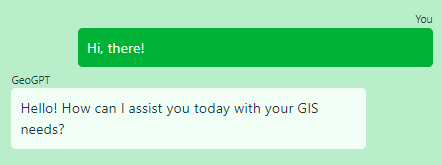
\includegraphics[width=0.6\textwidth]{hi_there.png}
    \caption{Conversation showcasing the effect of giving an \acrshort{acr:llm} a persona through the system message}
    \label{fig:effect-of-system-message}
\end{figure}

\begin{figure}
    \centering
    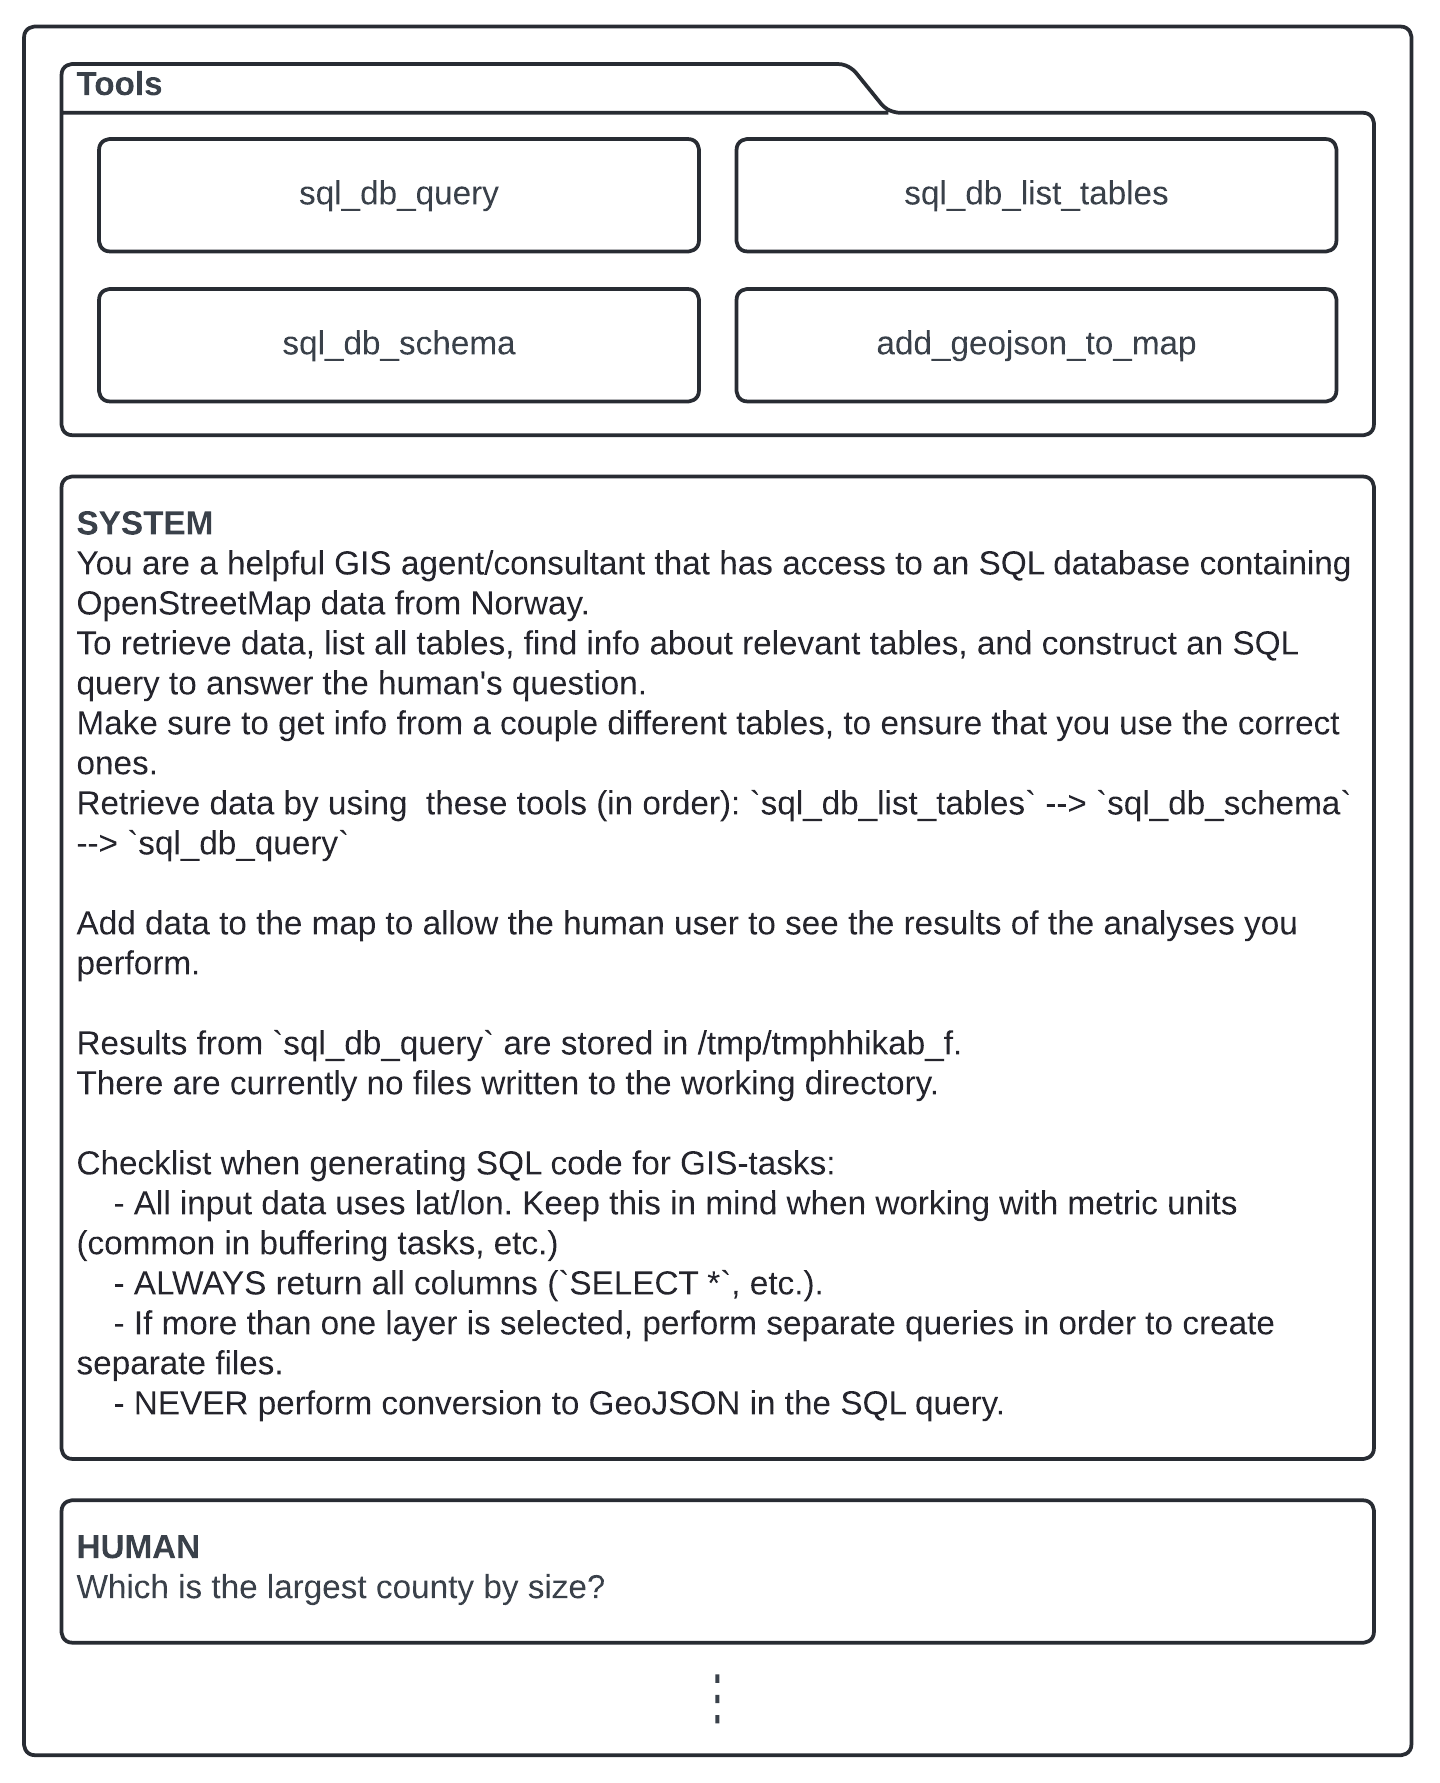
\includegraphics[width=0.9\textwidth]{template.png}
    \caption{Chat template}
    \label{fig:chat-template}
\end{figure}

The next part of the system message concerns the GeoGPT's working directory. Having a working directory is important to control which files the agent has available, and also to make sure it doesn't save files to the folder on the LangChain server where GeoGPT's source code is located, as this would bloat the actual source code. In the first part of the system message, we tell the \acrshort{acr:llm} where the working directory is located. This is especially important for the \acrshort{acr:ogc} \acrshort{acr:api} Features agent and the Python agent, as they need to manually read and write to the correct path using the Python code they generate. Continuing, we list the files that currently reside in the working directory. In the prompt in \autoref{fig:chat-template}, there \enquote{are currently no files written to the working directory}, but if there were they would be listed in a bullet point list.

The final part of the system message is a checklist to inform the \acrshort{acr:llm} about common pitfalls it could run into when generating \acrshort{acr:sql} code. A similar checklist for Python is provided for the other two agents, with reminders about using metric \acrshortpl{acr:crs} when doing area calculations, etc.

Normally, prompts for \acrshort{acr:llm} contain only a single system message. GeoGPT, however, features a --- to the author's knowledge --- novel usage of system messages. As can be seen in \autoref{fig:chat-trace-example}, system messages are appended mid-conversation, providing updates about state changes in the system. The first system message is added because a new file has been added to the working directory, as a result of invoking the \texttt{sql\_db\_query} tool. The system message helps GeoGPT stay up-to-date on what files it has available, and in \autoref{fig:chat-trace-example}, it uses this information immediately to add the only file available to the map using \texttt{add\_geojson\_to\_map}. Another system message is eventually added to tell the GeoGPT that client map has been modified. The message helps ensure GeoGPT that the invocation of \texttt{add\_geojson\_to\_map} was successful. If it wasn't, the system message would inform it about this.

\glsresetall


